\section{Introduction} \pagenumbering{arabic} \setcounter{page}{1}

\vspace{1cm}

\begin{figure}[h]
  \label{fig:paradise} \centering
\fcolorbox{black}{white}{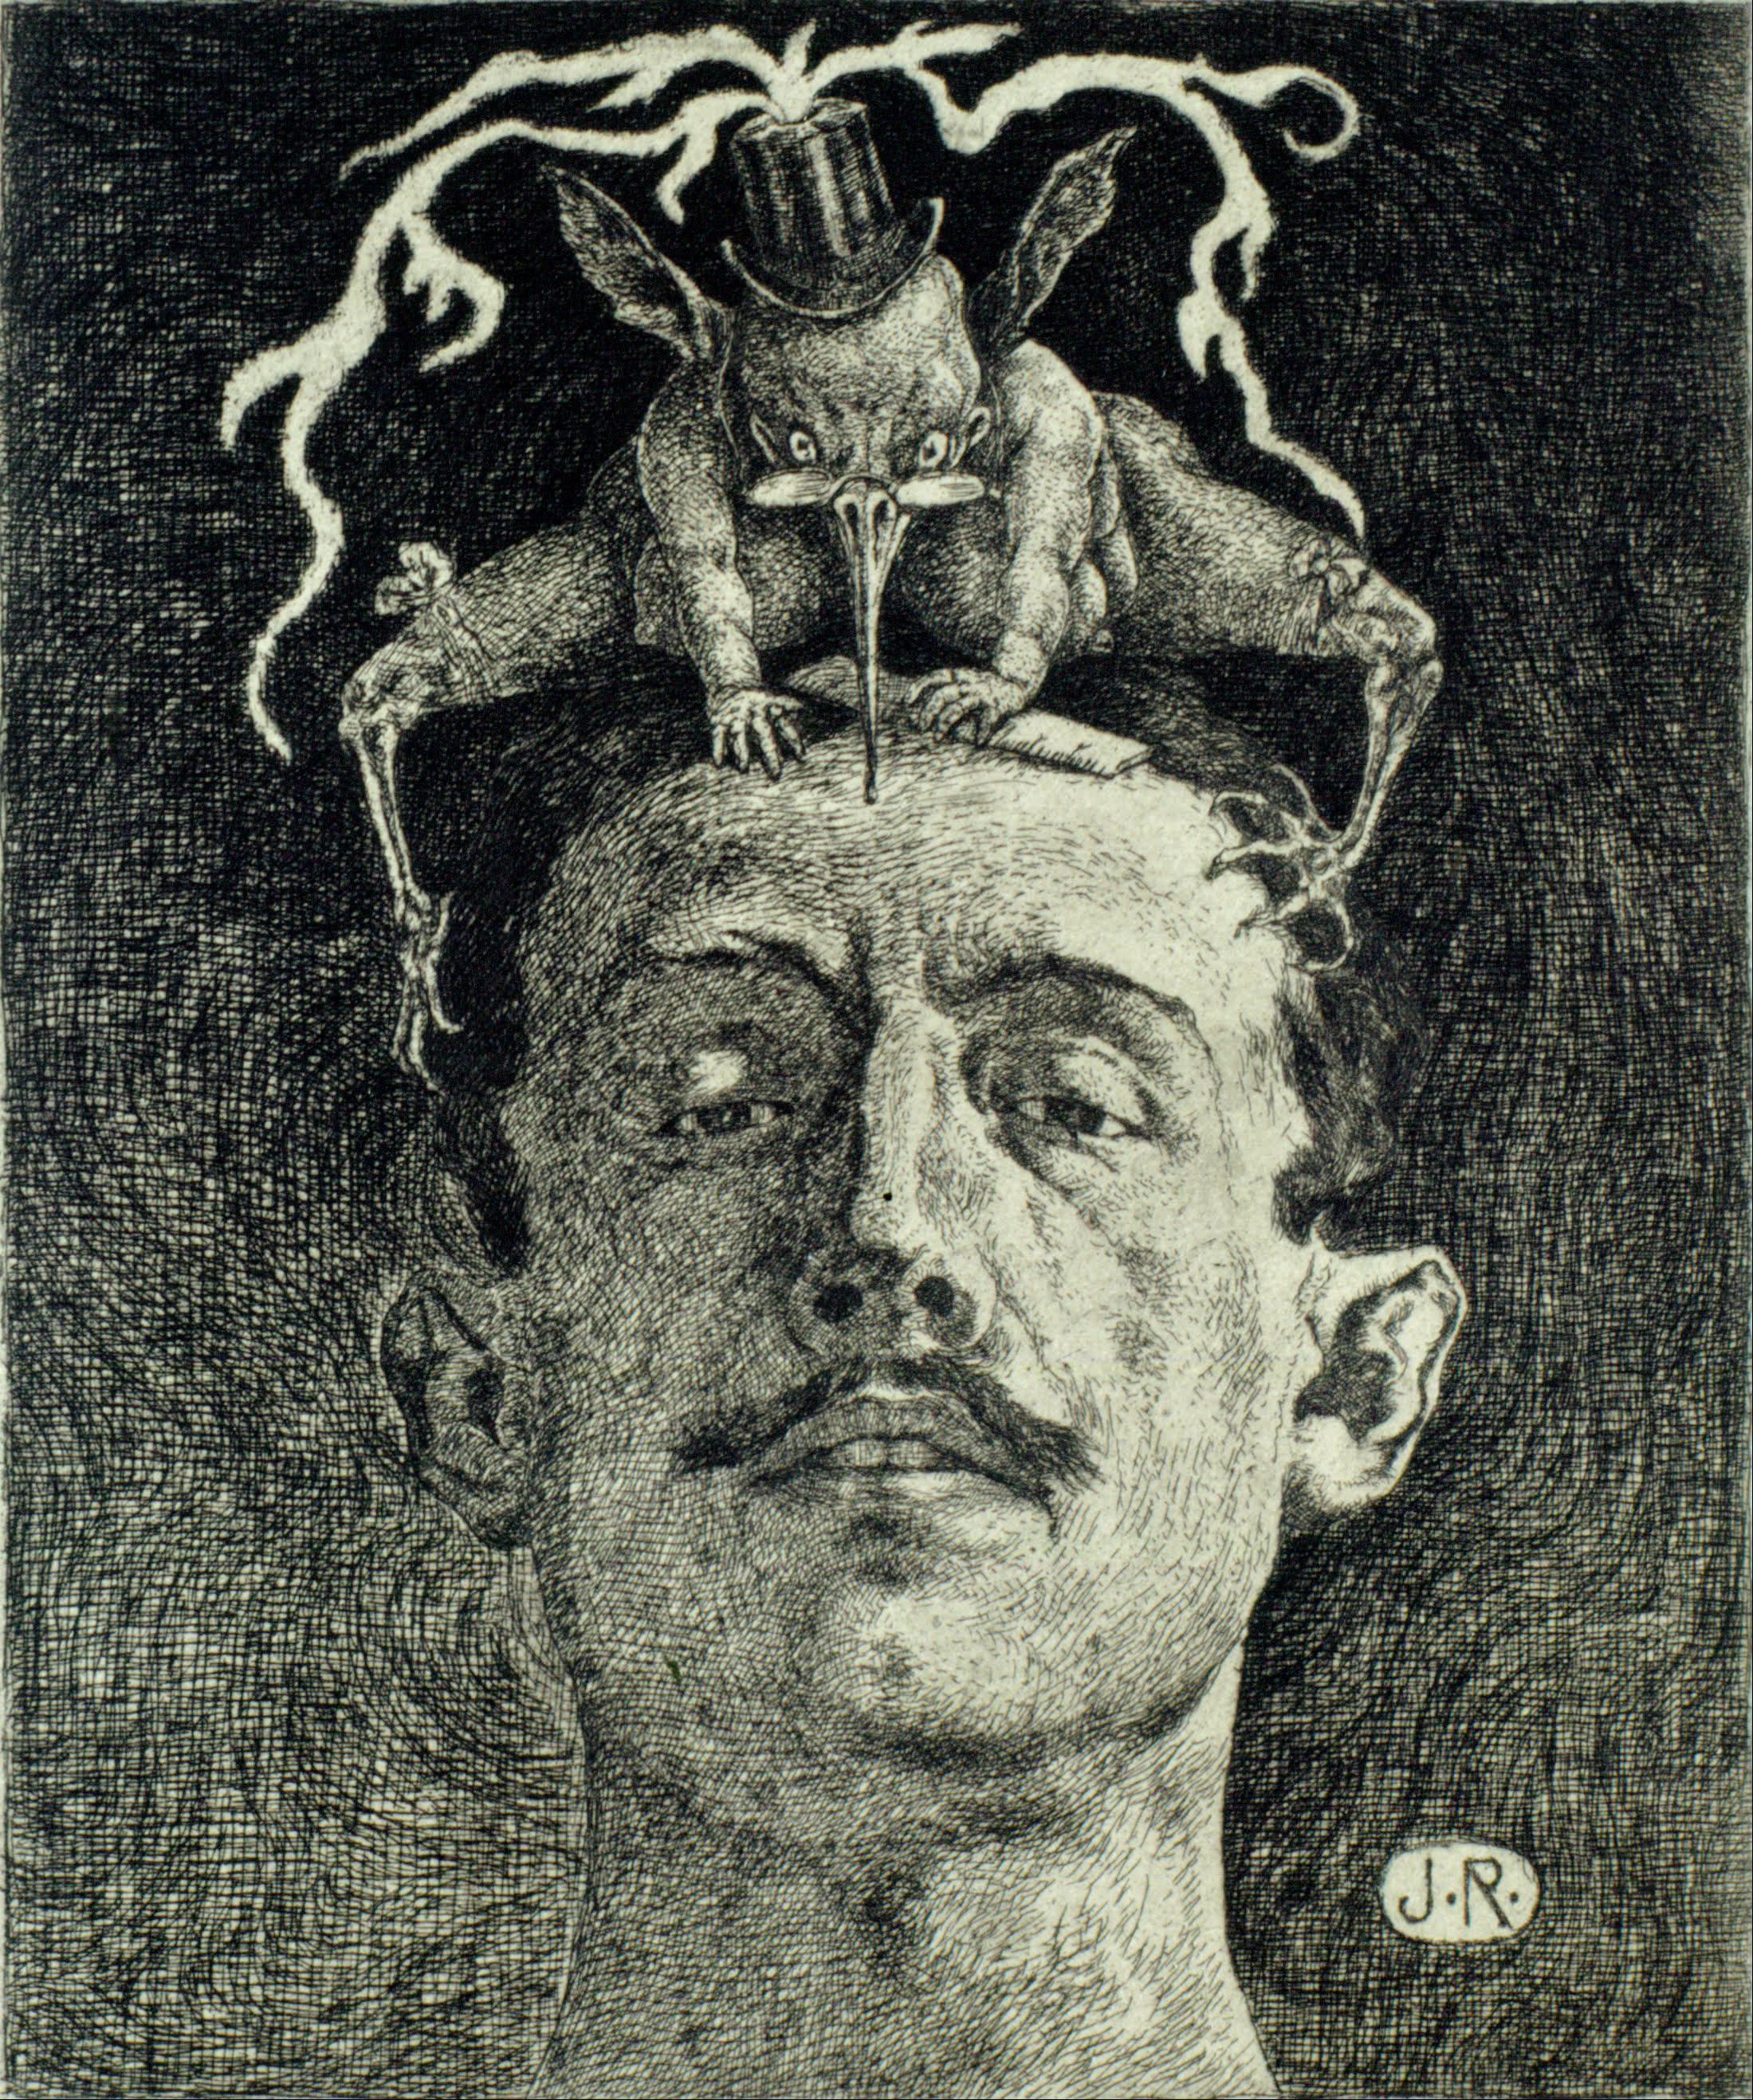
\includegraphics[width=0.3\textwidth]{innercritic}}
  \caption{Crítica by Julio Ruelas, ca. 1907}
\end{figure}

\vspace{1cm}

\lettrine[lines=3]{\Royal T}{his is an exposition on the theory of the
GAN algorithm}, otherwise known as \textit{generative adversarial
networks}. The GAN algorithm's name is descriptive in that the goal of
the algorithm is to produce a generative model, called a
\textit{generator}, through a two-player game with an adversary called
a \textit{discriminator}.

\begin{definition}
  \label{def:generator} Let $\Phi \subset \R^k$ be a space of
parameter values. A \textbf{generator} $\G$, parameterized by $\phi
\in \Phi$, is a function $G: \Phi \times \&Z \mapsto \target$, which
maps $\*z$ drawn from $\&Z$ according to $\pz$ to $\target$.
\end{definition}

\begin{definition}
  \label{def:discriminator} Let $\Theta \subset \R^k$ be a space of
parameter values. A \textbf{discriminator} $\D$, parameterized by
$\theta \in \Theta$, is a function $D: \Theta \times \target \mapsto
\R$, which compute the probability that $\*x$ was drawn from $\&X$
according to $\pt$.
\end{definition}

The purpose of a generative model is to generate samples from a high
dimensional space wherein the latent probability distribution is
intractible and other methods, such as Markov chain Monte-Carlo
(MCMC), are inadequate. Many use cases for GANs are in the generation
of photo-realistic images.

Other use cases include medical imaging, where data sets often suffer
from class imbalances since it is easier to find data on healthy
subjects. GANs have been used to augment data sets by producing
synthetic images of diseased plant and animal tissues as in
\cite{ref:nazki-2018}, \cite{ref:valerio-2017}, and
\cite{ref:frid-2018}. Synthetic data may also help anonymize sources
of data for medical research, as explored in \cite{ref:shin-2018}.

While most research focuses on the generative side of the algorithm,
it is worth keeping in mind that the GAN algorithm also produces a
discriminator, which is a classifier between two classes and has been
used as a classifier in \cite{ref:cortes-2017} to classify different
plant diseases, which was inspired by \cite{ref:odena-2016}.  The GAN
algorithm is a framework for training a generative model and comprises
two \textit{artificial neural networks}, a class of function made by
composing many primitive functions.

\subsubsection*{Neural Networks}

The structure of a neural network is defined by a directed graph (the
computations flow in a predetermined direction). At each node is a
composition of linear (or affine) functions with a nonlinear
activation function. The input and output of the nodes are determined
by the connectivity of the graph.

\begin{figure}[H] \centering
  \begin{tikzpicture} \tiny
    %%% Nodes.
    \begin{scope}[]
      \matrix[nodes = {draw, nn}, column sep = 0.5cm] {
        \node (q1) {$q_1$}; &
        \node (q2) {$q_2$}; &
        \node (q3) {$q_3$}; &
        \node (q4) {$q_4$}; &
        \node (q5) {$q_5$}; \\
      };
    \end{scope}
    \begin{scope}[yshift = -1cm]
      \matrix[nodes = {draw, nn}, column sep = 0.5cm] {
        \node (r1) {$r_1$}; &
        \node (r2) {$r_2$}; &
        \node (r3) {$r_3$}; &
        \node (r4) {$r_4$}; \\
      };
    \end{scope}
    \begin{scope}[yshift = -2cm]
      \matrix[nodes = {draw, nn}, column sep = 0.5cm] {
        \node (s1) {$s_1$}; &
        \node (s2) {$s_2$}; &
        \node (s3) {$s_3$}; & \node (s4) {$s_4$}; \\
      };
    \end{scope}
    \begin{scope}[yshift = -3cm]
      \matrix[nodes = {draw, nn}, column sep = 0.5cm] {
        \node (x1) {$x_1$}; &
        \node (x2) {$x_2$}; &
        \node (x3) {$x_3$}; &
        \node (x4) {$x_4$}; \\
      };
    \end{scope}
    \begin{scope}[yshift = -4cm]
      \matrix[nodes = {draw, nn}, column sep = 0.5cm] {
        \node (y1) {$y_1$}; &
        \node (y2) {$y_2$}; &
        \node (y3){$y_3$}; \\
      };
    \end{scope}
    \begin{scope}[yshift = -5cm]
      \matrix[nodes = {draw, nn}, column sep = 0.5cm] {
        \node (z1) {$z_1$}; &
        \node (z2) {$z_2$}; &
        \node (z3) {$z_3$}; &
        \node (z4) {$z_4$}; &
        \node (z5) {$z_5$}; \\
      };
\end{scope}

%%% Edges.
\foreach \q in {1, 2, 3, 4, 5} {
  \foreach \r in {1, 2, 3, 4} {
    \path [line] (q\q) -- (r\r);
  }
}

\foreach \r in {1, 2, 3, 4} {
  \foreach \s in {1, 2, 3, 4} {
    \path [line] (r\r) -- (s\s);
  }
}

\foreach \s in {1, 2, 3, 4} {
  \foreach \x in {1, 2, 3, 4} {
    \path [line] (s\s) -- (x\x);
  }
}

\foreach \x in {1, 2, 3, 4} {
  \foreach \y in {1, 2, 3} {
    \path [line] (x\x) -- (y\y);
  }
}

\foreach \y in {1, 2, 3} {
  \foreach \z in {1, 2, 3, 4, 5} {
    \path [line] (y\y) -- (z\z);
  }
}
  \end{tikzpicture}
  \caption{A Deep Neural Network}
  \label{fig:deep_nn}
\end{figure}

If we let $f_\theta$ denote the neural network parameterized by
$\theta$, we can think of training $f_\theta$ as searching through
$\Theta \subset [0, 1]^n$, the space of all possible
parameterisations, in search of $\theta$ that minimizes some
differentiable measure of loss.

An information theoretic explanation for what deep learning is and how
the training works is given in \cite{ref:tishby-2015} and
\cite{ref:tishby-2017}. Tishby touches on some important topics in
deep learning from an information theory perspective.  One such
assertion of his is the arbitrary nature of the structure of the
graph, i.e.\ there are many equivalent graphs that do the same thing;
the weights at each node do not have meaning. Therefore we are not
searching for some perfect $\theta^* \in \Theta$, as there are many
equivalent $\theta$.

There are many optimization algorithms for searching $\Theta$, most of
which are variations of gradient descent. Gradients are taken with
respect to the loss function $\&L$ and blame is distributed throughout
the graph by the \textit{backpropagation} algorithm. Backpropagation
was introduced in \cite{ref:rumelhart-1986}, and is essentially an
application of the chain rule of calculus to compute the derivatives
of the loss function with respect to each parameter in the graph.

\begin{figure}[H] \centering
  \begin{tikzpicture}
    \begin{scope}[] \matrix[] {
        \node (x1) {$x_1, x_2, \cdots, x_n$}; \\
      };
    \end{scope}
    %%% Summation:
    \begin{scope}[xshift = 3cm]
      \matrix[column sep = -0.2cm] {
        \node (p) {}; &
        \node (sum) {\large $\sum_{i = 1}^n x_i\theta_i - b$}; \\
      };
    \end{scope}
    %%% Activation:
    \begin{scope}[xshift = 5.5cm]
      \matrix[column sep = 1cm] {
        \node (sigma) { \Large ${1 \over 1 + e^{-x}}$}; \\
      };
    \end{scope}
    \path [line] (x1) -- (p); \path [line] (sum) -- (sigma);
  \end{tikzpicture}
  \caption{A Neuron}
  \label{fig:node_of_nn}
\end{figure}

Like a neural network, a linear regression model is a function
parameterized by a set of learnable weights $\theta$. The formula for
linear regression is
\begin{align}
  \label{eq:lin-reg} \hat{y} = \sum_{k=1}^m x_k\theta_k - b.
\end{align} The weight vector $\theta$ of a linear regression model
can be thought of as an expression for how important each entry of
$\mathbf{x}$ is for a specific output $y$. A linear regression model
may also include a bias term $b$, which in the case of a neural
network can be interpreted as the activation threshhold for the
neuron. In a sense, a neural network provides a way to compose many
linear regression models into a much larger
model. \cite{ref:cheng-2018} even go so far as to say that
feed-forward neural networks are equivalent to polynomial regression.

\subsubsection*{Generative Adversarial Networks}

The GAN algorithm comprises two neural networks, the generator $\G$
(and its parameters $\phi$) and the discriminator $\D$ (and its
parameters $\theta$). The generator's parameters $\phi$ are optimized
until $\G$ maps points from a space $\&Z$ to the desired region of
$\&X$ (the sample space). The discriminator's task is more
complicated. $\D$ is optimized until it can correctly classify samples
$\*x$ as either real or fake. $\D$ does this by calculating the
probability that the samples it observes came from true the
distribution $\pt$.

\begin{figure}[H] \centering
  \label{fig:simple_deep_nn} \tiny
  \begin{tikzpicture}[scale = 0.9]
    \begin{scope}
      %%% Noise:
      \begin{scope}[xshift = -5cm] \large
        \node (noise) {$\mathbf{z} \sim p_\mathbf{Z}(\mathbf{z})$};
      \end{scope}
      %%% Transformed Noise
      \begin{scope}[xshift = 1.5cm] \large
        \node (Gz) {$G(\mathbf{z})$};
      \end{scope}
      %%% Transformed Noise
      \begin{scope}[xshift = 4.5cm] \large
        \node (data) {$\mathbf{x} \sim p^*(\mathbf{x})$};
      \end{scope}
      %%% Generator.
      \begin{scope}[xshift = 0.4cm]
        \node (g_output) {};
      \end{scope}
      \begin{scope}[]
        \matrix[nodes = {draw, nn}, row sep = 0.3cm] {
          \node (q1) {}; \\
          \node (q2) {}; \\
          \node (q3) {}; \\
          \node (q4) {}; \\
        };
      \end{scope}
      \begin{scope}[xshift = -1cm]
        \matrix[nodes = {draw, nn}, row sep = 0.2cm] {
          \node (r1) {}; \\
          \node (r2) {}; \\
          \node (r3) {}; \\
          \node (r4) {}; \\
        };
      \end{scope}
      \begin{scope}[xshift = -2cm]
        \matrix[nodes = {draw, nn}, row sep = 0.2cm] {
          \node (s1) {}; \\
          \node (s2) {}; \\
          \node (s3) {}; \\
          \node (s4) {}; \\
        };
      \end{scope}
      \begin{scope}[xshift = -3.4cm]
        \node (g_input) {};
      \end{scope}
      \begin{scope}[xshift = -3cm]
        \matrix[nodes = {draw, nn}, row sep = 0.3cm] {
          \node (x1) {}; \\
          \node (x2) {}; \\
          \node (x3) {}; \\
          \node (x4) {}; \\
        };
      \end{scope}

      %%% Edges.
      \foreach \q in {1, 2, 3, 4} {
        \foreach \r in {1, 2, 3, 4} {
          \path [line] (r\r) -- (q\q);
        }
      }
      \foreach \r in {1, 2, 3, 4} {
        \foreach \s in {1, 2, 3, 4} {
          \path [line] (s\s) -- (r\r);
        }
      }
      \foreach \s in {1, 2, 3, 4} {
        \foreach \x in {1, 2, 3, 4} {
          \path [line] (x\x) -- (s\s);
        }
      }

      %%% Discriminator.
      \begin{scope}[xshift = 3cm, yshift = -1.7cm]
        \begin{scope}[yshift = 0.3cm]
          \matrix[column sep = 0.4cm] {
            \node (d_input_1) {}; &
            \node (d_input_2) {}; \\
          };
        \end{scope}
        \begin{scope}[]
          \matrix[nodes = {draw, nn}, column sep = 0.3cm] {
            \node (q1) {}; &
            \node (q2) {}; &
            \node (q3) {}; &
            \node (q4) {}; \\
          };
        \end{scope}
        \begin{scope}[yshift = -1cm]
          \matrix[nodes = {draw, nn}, column sep = 0.2cm] {
            \node (r1) {}; &
            \node (r2) {}; &
            \node (r3) {}; \\
          };
        \end{scope}
        \begin{scope}[yshift = -1.8cm]
          \matrix[nodes = {draw, nn}, column sep = 0.2cm] {
            \node (s1) {}; & \node (s2) {}; \\
          };
        \end{scope}
        \begin{scope}[yshift = -2.4cm]
          \matrix[nodes = {draw, nn}, column sep = 0.2cm] {
            \node (x1) {}; \\
          };
        \end{scope}

        \begin{scope}[yshift = -2.8cm]
          \node (d_output) {};
        \end{scope}

        %%% Edges.
        \foreach \q in {1, 2, 3, 4} {
          \foreach \r in {1, 2, 3} {
            \path [line] (q\q) -- (r\r);
          }
        }
        \foreach \r in {1, 2, 3} {
          \foreach \s in {1, 2} {
            \path [line] (r\r) -- (s\s);
          }
        }
        \foreach \s in {1, 2} {
          \foreach \x in {1} {
            \path [line] (s\s) -- (x\x);
          }
        }
      \end{scope}

      \begin{scope}[xshift = 3cm, yshift = -5.5cm]
        \large \node (p) {$D(G(\*z))$};
      \end{scope}

      \path [line] (noise) -- (g_input);
      \path [line] (g_output) -- (Gz);
      \path [line] (Gz) -- (d_input_1);
      \path [line] (data) -- (d_input_2);
      \path [line] (d_output) -- (p);

    \end{scope}
  \end{tikzpicture}
  \caption{The Architecture of the GAN Algorithm}
\end{figure}

The generator of the GAN algorithm trains a \textit{generative model},
which we define as any mathematical or statistical model that mimics
the process of creating the observed data \cite{ref:bishop}. Starting
with randomly initialized parameters, which means we randomly choose a
$\theta \in \Theta$, we optimize the model until it maps random input
into the desired output with frequencies similar enough to the desired
probability distribution. In other words we take a random vector $\*Z
= \left\{Z_1, Z_2, \dots, Z_n\right\}$, where each $Z_i \sim
\mathcal{N}(0, 1)$ is a normally distributed random variable with mean
0 and variance 1 (we could also use a random input following a
different distribution).
\begin{align}
  \label{eq:gen-model} f_\theta(\*Z): \*Z \mapsto \&X
\end{align} We then pass $\*Z$ through a parametric function which
does the transformation, and we obtain a sample from the target space
$\&X$.

The earliest reference to two-player games that result in the
production of a generative model can be found in \cite{ref:doyle}, a
short article containing the following game. \textit{``We are told the
constraints, we pick a distribution, God gets to pick the `real'
distribution, satisfying the constraints of course. Some disinterested
party picks an outcome according to the `real' distribution that God
has just picked, and we have to pay according to how surprised we are
to see that outcome.''} This is not quite the GAN algorithm, but it
has a similar moral, that is we seek a probability distriution and we
learn what qualities define it through feedback. If we iterate the
above procedure and formalize a way of learning from our surprise, we
arrive at something resembling the GAN algorithm.

As for the history of adversarial games (where the players are trying
to undermine each other), J\"{u}rgen Schmidhuber wrote more than one
paper, the first of which appeared in 1992, on what he called
``predictability minimization'', which is very similar to the GAN
algorithm (see \cite{ref:schmidhuber-1992} and
\cite{ref:schmidhuber-2018}). The idea behind \textit{predictability
minimization} was for one player to try to predict outcomes in some
event space and the adversary tries to minimize the ability of that
player to make those predictions.

A blog post from 2010 essentially describes the GAN algorithm, see
\cite{ref:niemitalo-2010}. In 2012, a paper on adversarial support
vector machines was written by \cite{ref:zhou-2012}. Finally, in 2014
an algorithm for training models to simulate the behaviour of animals
based on two populations, replicas and classifiers, was written by
\cite{ref:li-2014}.

In 2014, while a student of Yoshua Bengio at the Universit\'{e} de
Montr\'{e}al, Ian Goodfellow and colleagues published
\textit{Generative Adversarial Nets}.  This paper has since inspired
many publications and has triggered a surge in the interest in
generative models.

%%% Local Variables: %%% mode: latex %%% TeX-master: "../thesis.tex"
%%% TeX-master: "../thesis"
%%% End:
